\documentclass{beamer}

\mode<presentation>
\usetheme{Pittsburgh}
\usecolortheme{whale}
\setbeamertemplate{section in toc}{\inserttocsectionnumber.~\inserttocsection}
\setbeamertemplate{subsection in toc}[subsections numbered]
\setbeamerfont{caption}{size=\tiny}
\beamertemplatenavigationsymbolsempty{}

\usepackage[utf8]{inputenc}
\usepackage[T1]{fontenc}
\usepackage[american]{babel}
\usepackage{cmbright}
\usepackage[scaled=0.85]{beramono}
\usepackage{multimedia}
\usepackage{hyperref}
\usepackage{graphicx}
\usepackage[round]{natbib}

\title{Modeling the sensation of fluctuation strength}
\author{Rodrigo García León
  \texorpdfstring{\\ M.Sc Student Human-Technology Interaction
  \\ \texttt{r.garcia.leon@student.tue.nl}}{}}
\institute{Department of Industrial Engineering \& Innovation Sciences
  \texorpdfstring{\\Eindhoven University of Technology}{}}
\date{\today}

\newcommand{\playbutton}{\raisebox{-1ex}{\hbox%
  {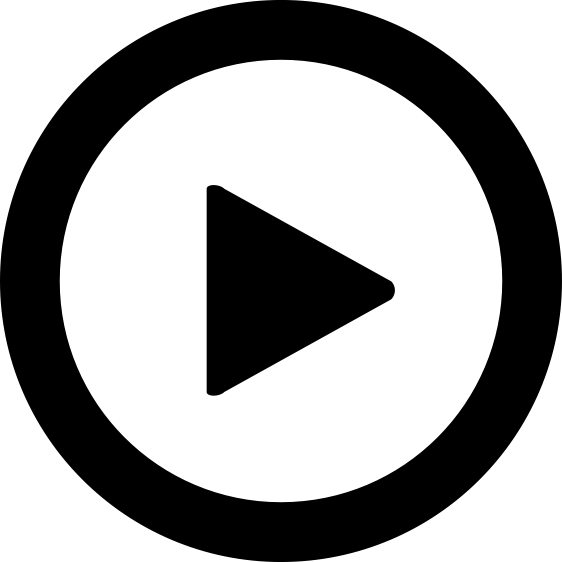
\includegraphics[height=18pt]{play}}}}
\newcommand{\addsound}[1]{
  \movie[label=#1]{}{#1.wav}
  \hyperlinkmovie{#1}{\playbutton}
}

\AtBeginSection[] {
  \begin{frame}
    \frametitle{Outline}
    \tableofcontents[currentsection]
  \end{frame}
}

\begin{document}

\frame{\titlepage}

\section*{Outline}
\begin{frame}
  \frametitle{Outline}
  \tableofcontents
\end{frame}

\section{Introduction}
\subsection{Perceptual Attributes}
\begin{frame}
  \frametitle{Perceptual Attributes}
  \begin{itemize}
    \item Discernible dimensions in which an auditory event can be decomposed
    \item Derived from physical characteristics of sounds (frequency, sound
      pressure level, etc.)
    \item Examples of them are: loudness, sharpness, roughness, fluctuations
      strength; among others.
    \item Allow to understand auditory events from a perceptual point of view
  \end{itemize}
\end{frame}

\subsection{Fluctuation Strength}
\begin{frame}
  \frametitle{Fluctuation Strength}
  \begin{itemize}
    \item Sensation that arises from modulated sounds with a slowly varying
      envelope (i.e., a modulation frequency $f_m < 20$ Hz)
    \item Envelope fluctuation can be amplitude-modulated (AM) or
      frequency-modulated (FM)
  \end{itemize}

  \begin{columns}
    \begin{column}{0.175\textwidth}
      \hbox{\hbox to 12mm{AM tone} \addsound{am}} \\
      \medskip
      { \scriptsize
        $f_m = 4$ [Hz] \\ $f_c = 1$ [kHz] \\
        SPL = 70 [dB] \\ $m_d = 40$ [dB] \\}
    \end{column}
    \begin{column}{0.175\textwidth}
      \includegraphics[height=0.25\textheight]{am_time}
    \end{column}
    \begin{column}{0.175\textwidth}
      \includegraphics[height=0.25\textheight]{am_frequency}
    \end{column}
  \end{columns}

  \vspace{2mm}

  \begin{columns}
    \begin{column}{0.175\textwidth}
      \hbox{\hbox to 12mm{FM tone} \addsound{fm}} \\
      \medskip
      { \scriptsize
        $f_m = 4$ [Hz] \\ $f_c = 1.5$ [kHz] \\
        SPL = 70 [dB] \\ $d_f = 700$ [Hz] \\}
    \end{column}
    \begin{column}{0.175\textwidth}
      \includegraphics[height=0.25\textheight]{fm_time}
    \end{column}
    \begin{column}{0.175\textwidth}
      \includegraphics[height=0.25\textheight]{fm_frequency}
    \end{column}
  \end{columns}
\end{frame}

\begin{frame}
  \frametitle{Fluctuation Strength and Roughness}
  \begin{itemize}
    \item Above $f_m > 20$ Hz the fluctuation strength sensation diminishes
      and the roughness sensation begins to take effect
  \end{itemize}

  \begin{columns}
    \begin{column}{0.175\textwidth}
      \hbox{\hbox to 24mm{Fluctuating tone} \addsound{am}} \\
      \medskip
      { \scriptsize
        $f_m = 4$ [Hz] \\ $f_c = 1$ [kHz] \\
        SPL = 70 [dB] \\ $m_d = 40$ [dB] \\}
    \end{column}
    \begin{column}{0.175\textwidth}
      \includegraphics[height=0.25\textheight]{am_time}
    \end{column}
    \begin{column}{0.175\textwidth}
      \includegraphics[height=0.25\textheight]{am_frequency}
    \end{column}
  \end{columns}

  \vspace{2mm}

  \begin{columns}
    \begin{column}{0.175\textwidth}
      \hbox{\hbox to 16mm{Rough tone} \addsound{rough}} \\
      \medskip
      { \scriptsize
        $f_m = 70$ [Hz] \\ $f_c = 1.5$ [kHz] \\
        SPL = 70 [dB] \\ $m_d = 40$ [dB] \\}
    \end{column}
    \begin{column}{0.175\textwidth}
      \includegraphics[height=0.25\textheight]{rough_time}
    \end{column}
    \begin{column}{0.175\textwidth}
      \includegraphics[height=0.25\textheight]{rough_frequency}
    \end{column}
  \end{columns}
\end{frame}

\begin{frame}
  \frametitle{Band-pass Characteristic}
  \begin{figure}
    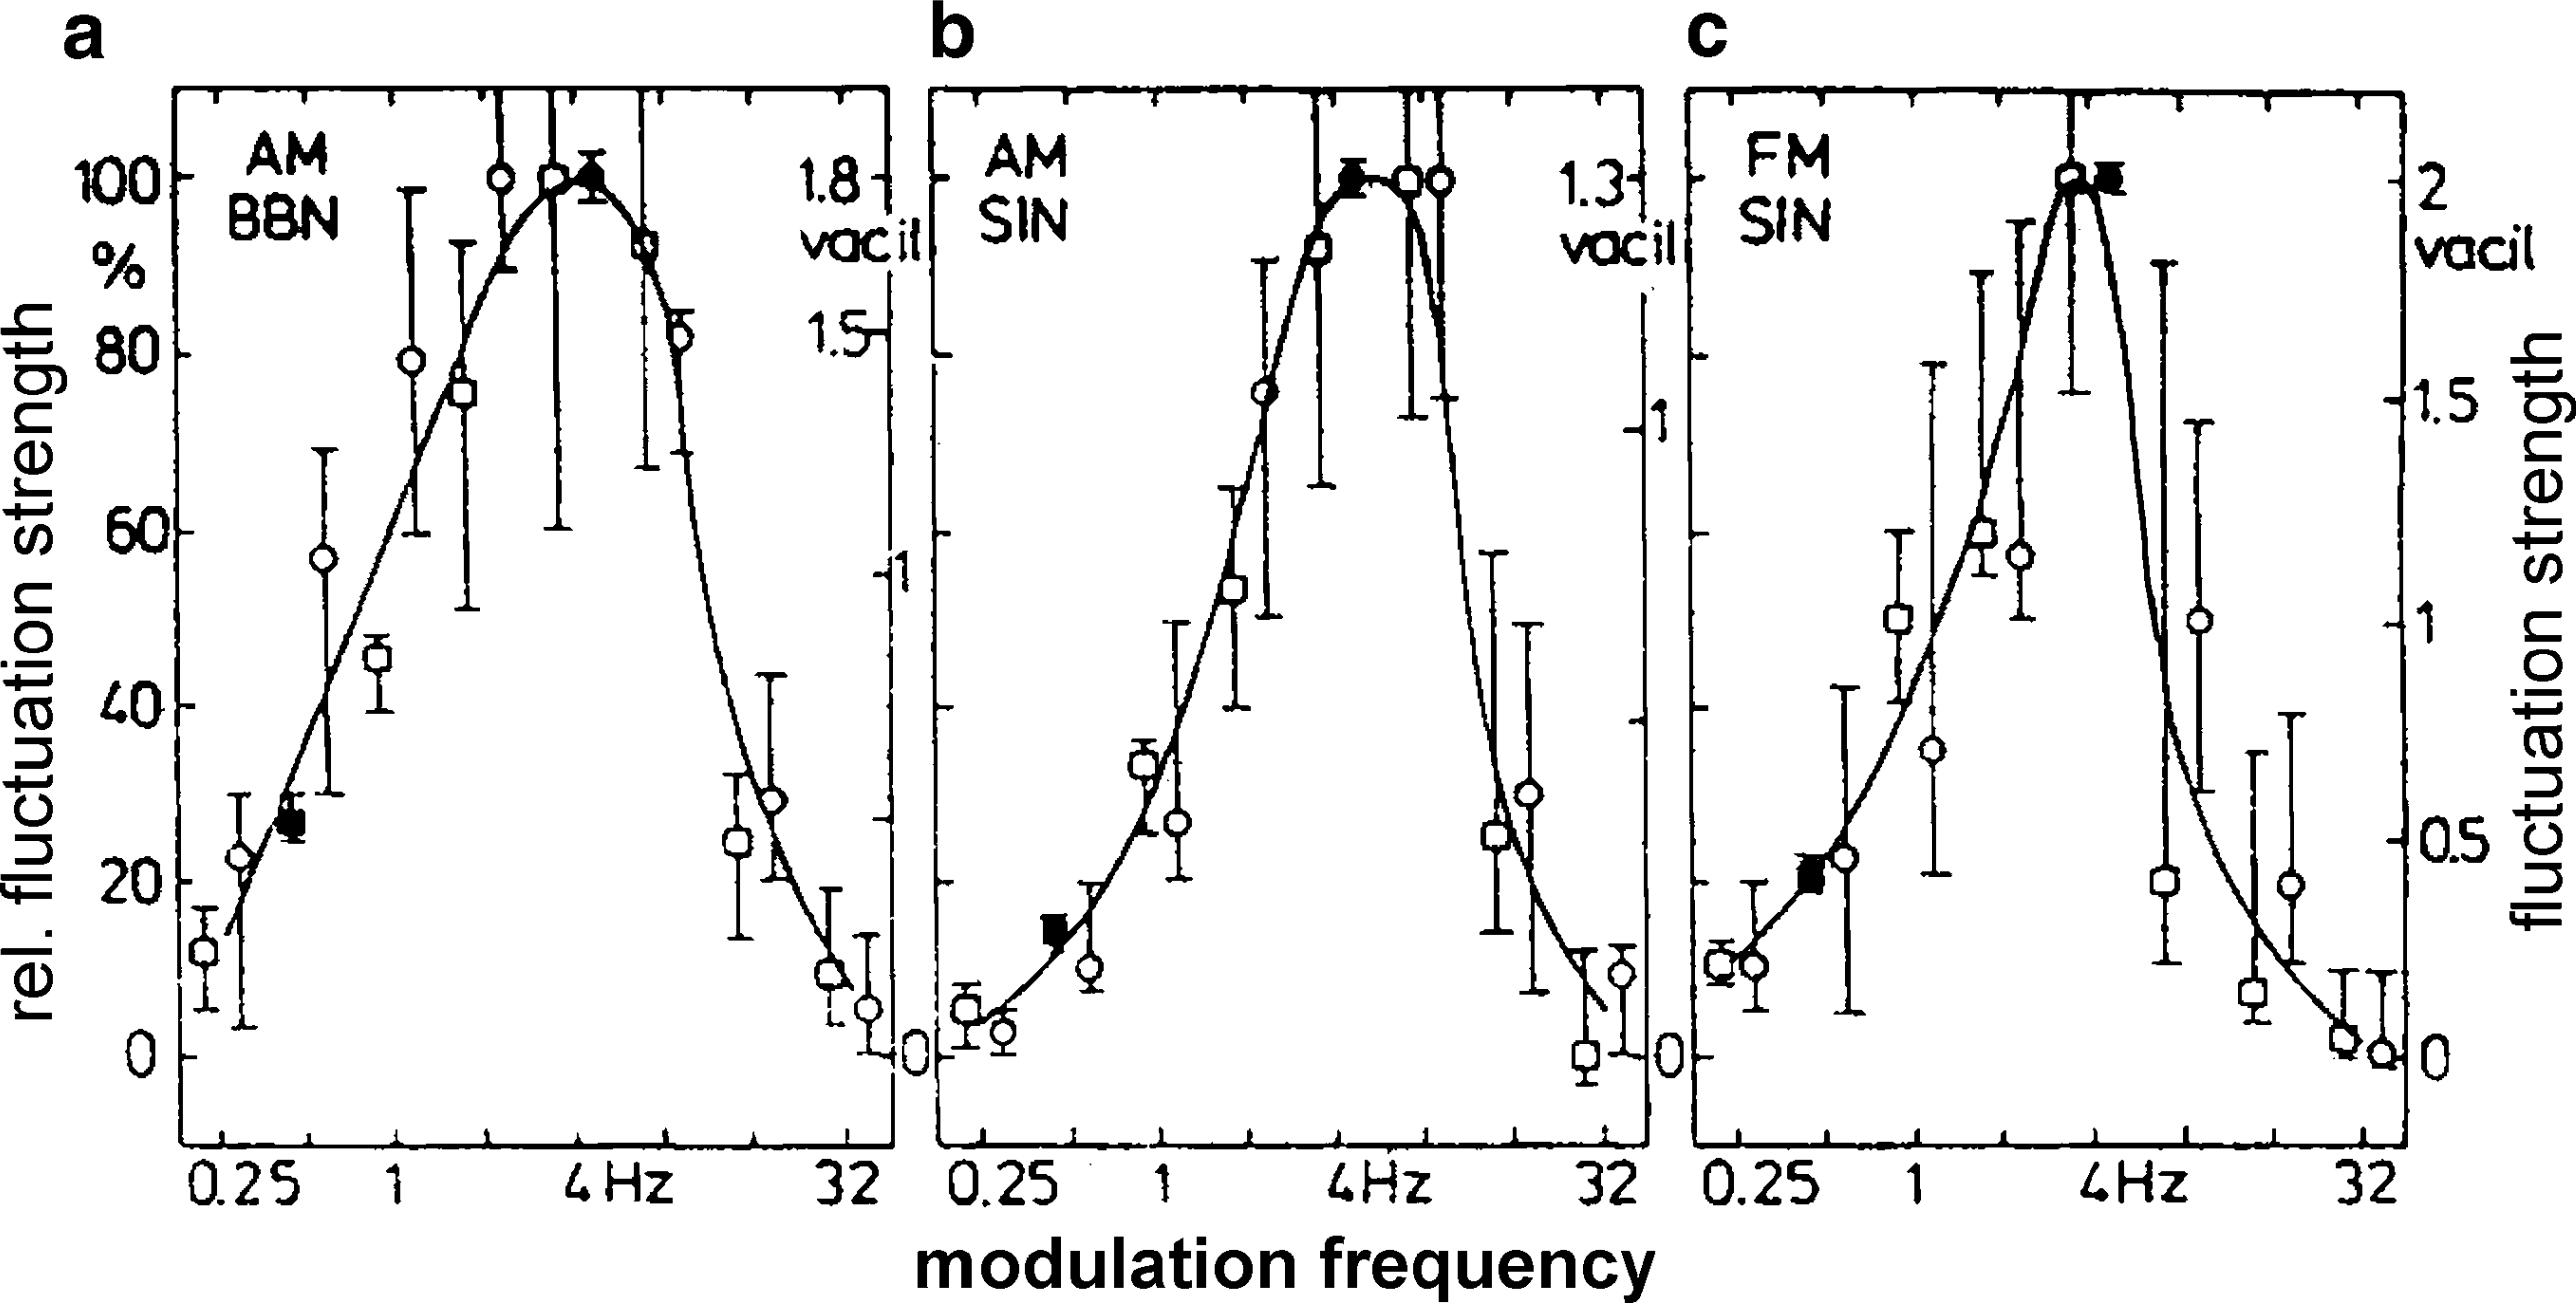
\includegraphics[width=\textwidth]{fs_vs_md}
    \caption{Fluctuation strength as a function of modulation frequency for: (a)
      amplitude-modulated broad-band noise, (b) amplitude-modulated tones and
      (c) frequency-modulated tones; as presented by
      \citet{Fastl2007Psychoacoustics}}
  \end{figure}
\end{frame}

\subsection{Current Research}

\begin{frame}
  \frametitle{Importance}
  \begin{itemize}
    \item Possible relation with the speech system
    \begin{itemize}
      \item Maximum fluctuation strength value occurs around $f_m = 4$ Hz
      \item Humans beings utter syllables at a rate of 4 syllables per second
    \end{itemize}
    \item Influences pleasantness of sounds
    \begin{itemize}
      \item Functionally (alarm signals)
      \item Musicality (instruments enjoyableness)
    \end{itemize}
  \end{itemize}
\end{frame}

\begin{frame}
  \frametitle{Rationale for Research}
  \begin{itemize}
    \item Methodological issues in past studies
    \begin{itemize}
      \item Unfamiliarity with fluctuation strength
      \item Confusion between roughness and fluctuation strength
    \end{itemize}
    \item Not widely available work when it comes to modeling the fluctuation
      strength sensation
  \end{itemize}
\end{frame}

\begin{frame}
  \frametitle{Objectives}
  \begin{itemize}
    \item Formulate a clear methodological procedure to eliminate problems
      found in past studies
    \item Propose a fluctuation strength model
    \begin{itemize}
      \item Based on existing roughness models
      \item Adjusted to collected experimental data
    \end{itemize}
  \end{itemize}
\end{frame}

\section{Experimental Design}
\subsection{Training Phase}
\subsection{Experimental Phase}

\section{Model Development}

\section{Discussion}


\section*{Credits}
\begin{frame}
  \frametitle{Credits}
  play \playbutton{} by Mike Ashley from the Noun Project
\end{frame}

\section*{Bibliography}
\begin{frame}<beamer:0>
  \bibliographystyle{plainnat}
  \bibliography{/Users/rodrigo/Library/texmf/tex/latex/References.bib}
\end{frame}

\end{document}
